%% Copernicus Publications Manuscript Preparation Template for LaTeX Submissions
%% ---------------------------------
%% This template should be used for copernicus.cls
%% The class file and some style files are bundled in the Copernicus Latex Package, which can be downloaded from the different journal webpages.
%% For further assistance please contact Copernicus Publications at: production@copernicus.org
%% https://publications.copernicus.org/for_authors/manuscript_preparation.html


%% Please use the following documentclass and journal abbreviations for preprints and final revised papers.

%% 2-column papers and preprints
\documentclass[journal abbreviation, manuscript]{copernicus}



%% Journal abbreviations (please use the same for preprints and final revised papers)


% Advances in Geosciences (adgeo)
% Advances in Radio Science (ars)
% Advances in Science and Research (asr)
% Advances in Statistical Climatology, Meteorology and Oceanography (ascmo)
% Annales Geophysicae (angeo)
% Archives Animal Breeding (aab)
% ASTRA Proceedings (ap)
% Atmospheric Chemistry and Physics (acp)
% Atmospheric Measurement Techniques (amt)
% Biogeosciences (bg)
% Climate of the Past (cp)
% DEUQUA Special Publications (deuquasp)
% Drinking Water Engineering and Science (dwes)
% Earth Surface Dynamics (esurf)
% Earth System Dynamics (esd)
% Earth System Science Data (essd)
% E&G Quaternary Science Journal (egqsj)
% European Journal of Mineralogy (ejm)
% Fossil Record (fr)
% Geochronology (gchron)
% Geographica Helvetica (gh)
% Geoscience Communication (gc)
% Geoscientific Instrumentation, Methods and Data Systems (gi)
% Geoscientific Model Development (gmd)
% History of Geo- and Space Sciences (hgss)
% Hydrology and Earth System Sciences (hess)
% Journal of Bone and Joint Infection (jbji)
% Journal of Micropalaeontology (jm)
% Journal of Sensors and Sensor Systems (jsss)
% Magnetic Resonance (mr)
% Mechanical Sciences (ms)
% Natural Hazards and Earth System Sciences (nhess)
% Nonlinear Processes in Geophysics (npg)
% Ocean Science (os)
% Polarforschung - Journal of the German Society for Polar Research (polf)
% Primate Biology (pb)
% Proceedings of the International Association of Hydrological Sciences (piahs)
% Scientific Drilling (sd)
% SOIL (soil)
% Solid Earth (se)
% The Cryosphere (tc)
% Weather and Climate Dynamics (wcd)
% Web Ecology (we)
% Wind Energy Science (wes)


%% \usepackage commands included in the copernicus.cls:
%\usepackage[german, english]{babel}
%\usepackage{tabularx}
%\usepackage{cancel}
%\usepackage{multirow}
%\usepackage{supertabular}
%\usepackage{algorithmic}
%\usepackage{algorithm}
%\usepackage{amsthm}
%\usepackage{float}
%\usepackage{subfig}
%\usepackage{rotating}


\usepackage{comment} 

\begin{document}

\title{Phydra 0.1: an open source Python library for flexible, modular and reproducible marine ecosystem modeling based on ordinary differential equations} 


% \Author[affil]{given_name}{surname}
\Author[1]{Benjamin}{Post}
\Author[1]{Esteban}{Acevedo-Trejos}
\Author[2]{Andrew }{Barton}
\Author[3]{Benoît}{Bovy}
\Author[1]{Agostino}{Merico}



\affil[1]{Leibniz Centre for Tropical Marine Research (ZMT), Bremen, Germany}
\affil[2]{Scripps Institution of Oceanography, La Jolla, CA, United States}
\affil[3]{GFZ German Research Centre for Geosciences, Potsdam, Germany}


%% The [] brackets identify the author with the corresponding affiliation. 1, 2, 3, etc. should be inserted.

%% If an author is deceased, please mark the respective author name(s) with a dagger, e.g. "\Author[2,$\dag$]{Anton}{Aman}", and add a further "\affil[$\dag$]{deceased, 1 July 2019}".

%% If authors contributed equally, please mark the respective author names with an asterisk, e.g. "\Author[2,*]{Anton}{Aman}" and "\Author[3,*]{Bradley}{Bman}" and add a further affiliation: "\affil[*]{These authors contributed equally to this work.}".


\correspondence{Benjamin Post (benjamin.post@leibniz-zmt.de)}


\runningtitle{phydra v1}

\runningauthor{Post}





\received{}
\pubdiscuss{} %% only important for two-stage journals
\revised{}
\accepted{}
\published{}

%% These dates will be inserted by Copernicus Publications during the typesetting process.

\firstpage{1}

\maketitle

\begin{abstract} [Just collecting ideas:] 

Marine ecosystem modeling is central to understanding the biogeochemical cycles driving the earth system. 

These models can have highly variable complexity, both in terms of mechanistic and spatial resolution. 
No consensus in terms of adequate model complexity and formulation has been reached, although there are many canonical model structures used and modified.

This paper introduces Phydra, an open-source library for marine ecosystem modeling built with the object-oriented modeling framework Xarray-simlab-ode (XSO), with the goal to support efficient, flexible and easily reproducible development of models based on ordinary differential equations. 

Phydra provides pre-built models and model components that can be modified and assembled to complex ecosystem models. 

All basic processes can be adapted and modified in simple Python to describe different and more complex ecosystems. The first release focuses on zero-dimensional phytoplankton models, but models of higher dimensionality are also possible.

Xarray data-structure, self-documenting workflow, ease of sharing models, as well as input and output.

Phydra is embedded in the Python scientific ecosystem and is natively compatible with many tools for prototyping, analysis \& visualisation of models.

This paper presents the general structure of Phydra, the usage of xarray-simlab-ode and the workflow of developing model applications of varying complexity.

Phydra, as well as all models and other work presented here is available open-source and can be used by the scientific community to build, modify, run and test ODE-based models. The Phydra standard library aspect, can collaborate share model functions mechanisms, really focus on science instead of fixing bugs.. 

Comprehensive documentation is available online.





% Through the combination of the XSO framework and the Phydra library, a high level of customisation and flexibility is combined with less boilerplate code and technical setup.

%Phydra is a Python package, embedded in the Python scientific ecosystem and is natively compatible with many tools for prototyping, analysis \& visualisation of models.

%, allowing modelers to simplify the model construction and focus on the scientific questions.

%Xarray-simlab-ODE provides a framework based on compact python classes and custom variables to define systems of ordinary or partial differential equations, that can be used with different solvers.


%Here, we demonstrate the usage of the phydra v1 package in a simple NPZD setting and to showcase the flexibility, in a more complex size based trophic structure model. Both in slab physics.

%The utility of the phydra package is here shown via three model implementations. Two models from literature are recreated, and the flexible nature of this package allows a combination of as a third example. 
\end{abstract}


\copyrightstatement{TEXT} %% This section is optional and can be used for copyright transfers.

%%% added Section for editing purposes, later simply use \introduction
\section{Introduction}
%\introduction  %% \introduction[modified heading if necessary]

% introduction should be adundantly clear with no unecessary details!
% can also mention open source, but just high-level summaries, same on phydra details, no detail in intro
% establish, why what you make is different from everything done before. why it is important! (2 sentences)

% 2nd Section:
% Background, theoretical framework. Specifics here!

% FIRST SECTION: general info - Biogeochemical role of phytoplankton

%- P1: why phytoplankton important?
\subsection{Models of marine ecosystems}
- major primary producers ocean ecosystem, understanding important, global change (important part of climate models)

These microorganisms form the basis of the food webs, and contribute roughly half of the oxygen in our atmosphere through photo- synthesis \citep{Field2009}.

The biomass produced indirectly feeds a considerable part of earth’s population through fisheries \citep{Stock2017} and also shapes the elemental composition of oceanic water itself \citep{Redfield1958}.

A small fraction of primary production sinks out of the photic layer as fecal pellets or detrital matter, to the deeper ocean, and an even smaller fraction reaches the sea floor as sediment (\~ 1 \%) and is finally removed from the system over geological times \citep{Honjo2008}. Carbon sequestered this way is removed from the ocean-atmosphere system for potentially millions of years.

- phytoplankton diversity 
Originating from several major phyla, there are estimated to be at least 25,000 species of phytoplankton \citep{Falkowski2004a} spanning over nine orders of magnitude in cell size \citep{Sieburth1978PelagicFractions, Finkel2010}.

- complex system --> complex models?! dealing with highly dimensional models \citep{Dutkiewicz2020DimensionsDiversity}


%  \subsection{Phytoplankton modeling: From NPZD to DARWIN}
%- P2: why people model phytoplankton? (what are the types of model we use? npzd, pft, size, darwin, etc.)
- based on ordinary diff equations!

- quote Gentleman history of marine ecosystem modeling \citep{Gentleman2003a}

- cite the beautiful paper on Steele's legacy \citep{Anderson2019RememberingEcosystems}

Given the complexity of the ocean ecosystem, it is necessary to aggregate our knowledge of the many smaller parts into comprehensive ecological models in order to understand the full-scale implications. Computational models of phytoplankton growth have been developed since the 1970s and have greatly increased in sophistication and complexity since then, co-evolving with the rise in computational resources. Ecosystem modelling started with simple box-model descriptions of a few trophic levels. These were the nutrient-phytoplankton-zooplankton (NPZ) and nutrient-phytoplankton-zooplankton-detritus (NPZD) models, which succeeded in reproducing the basic bloom dynamics observed in the temperate ocean \citep{Evans1985ACycles, Fasham1990a}. 

% \subsection{Running before we can walk}
% INSTEAD OF SUBSECTIONS; THESE ARE SIMPLY PARAGRAPHS

%- P3: all these different models, what is the problem? [Motivation for a better toolkit]
The simplicity of an NPZD model, where each of the four ecosystem components is represented by a single state variable, can be criticised as oversimplifying the complexity of a natural plankton community.

- These are very simplistic descriptions of ocean ecosystems, these models unavoidably limit the characterization of a diverse phytoplankton community [citation of Bruggeman?]. 

To make up for this shortcoming, in the following two decades, these models were expanded to more complex plankton functional type (PFT) models \citep{LeQuere2005}. For every group of species that fulfil a distinct ecosystem function, a new set of state variables and parameters was added, complicating the model structure and massively prolonging calculations. This somewhat intuitive approach of having every functional group represented in a model, however, did create problems. First and foremost, this is the lack and inherent uncertainty of data from field and culture experiments to constrain functional types. This again leads to the difficulty of validating the model output in light of insufficient information \citep{Shimoda2016}.

- Complex PFT models should not be initialized naively, but instead treated as hypotheses and multiple structures and levels of complexity should be tested against objective functions (usually data). \citep{Franks2009}

- Parameter identification in marine ecosystem models is complicated, but very important! \citep{Schartau2017}

- misleading legacies in phytoplankton modeling, formulations are routinely used that do not make physiological sense \citep{Smith2014}

and state: phydra is built with the idea in mind, that all ecosystem models are theories/hypotheses, that need to be tested against data, and tested against other models (particularly models of varying complexity). Occam's razor. 

- lots of models, in lots of (often old) programming languages, varying implementations
- all different, hidden (+very complex) codebase, not easy to adapt \& modify

ALTHOUGH, actually often very similar in nature and underlying technical processes, so if we could use a common framework that is sufficiently accessible and flexible, we can spend much less time on technicalities.

- but development in data science \& other computer science areas, towards reproducible tools, towards shared frameworks and capabilities (like Benoît said in his blog post: \href{https://medium.com/pangeo/pangeo-data-and-models-280b251ff0cd}{LINK} )

- tools should foster scientific collaboration
"easy to use, open source, easy to modify, toolbox"
- python Pangeo software ecosystem (jupyter, xarray, zarr)


\subsection{Open, flexible \& collaborative modeling}

%\subsection{Collaborative modelling using open source solution}
%- P4: Here's my solution! Here I present flexible model framework. explain basic structure and function

% can also mention open source, but just high-level summaries, same on phydra details, no detail in intro
% establish, why what you make is different from everything done before. why it is important! (2 sentences)

The tools used in academic computational modeling show a growing gap to the software ecosystems for data analysis. Perhaps in part due to the smaller user base, the former often have a steeper learning curve, are less accessible to novice users and can result in convoluted workflows. The latter is evolving rapidly towards more interactive and streamlined workflows.

Implementations of marine ecosystem models often evolve organically to higher complexities at the expense of their readability, which may compromise sustainability in the long term. In particularly, simplifying already complex models is not always simple and easy.

There are already some great modeling frameworks aimed to address the two issues above in the Python Scientific ecosystem (e.g., Climlab, CliMT/Simpl, Landlab), but there is to our knowledge no project to establish such a modeling framework in marine ecosystem modeling. \textit{[Not sure if this is true!]}

There have been different projects aimed at increasing the ease of model creation, both on the lower and higher-end. All projects have trade-offs, and what is most important is a common language and communication within the user community.
There are these.. and these projects (need some examples: Ecosym (?), Stella modeling tool (GUI), etc.).
Some of these proprietary software = not good!

Phydra is not designed to be specifically used with a graphical user interface (GUI), although such functionality could be added to the modular code base.
The design aims at allowing intuitive control of all levels of complexity, the base python code, mathematical solver implementations, as well as the higher level of assembling models from building blocks.

Why python? -> most popular programming language, rich scientific user community, Pangeo, rising language, relatively easy to learn

"Python is a high-level programming language well suited to rapid development and prototyping, as well as being more accessible to domain scientists than low-level languages such as FORTRAN or C++." - Mobius GMD paper
- This is also due to the dynamic interpretation of python, which makes python slower, but python is rapidly developing and leveraging other lower level language for speed. Also has growing functionality for parallelisation of code execution which is very relevant to large multi-dimensional marine ecosystem model use cases. 

Many large physical and ecological models are to this day written in FORTRAN. Due to the statically-typed nature it is more computationally efficient particularly for larger models. Yet despite it's speed, FORTRAN remains less accessible to scientists and usage and literacy of Python in the scientific community far exceeds that of FORTRAN.
Phydra is a project to bridge the gap between older, but more efficient ecosystem model code written in low-level languages like C++ and FORTRAN and the flexibility and usability of modern high-level programming languages. Python is a free and open-source language that is flexible, popular and has gained wide use in the scientific community. By being written in Python, Phydra can interact with a rich environment of popular scientific and numerical packages, and e.g. tool for machine learning. 


\subsection{Aims}
% AIM for phydra:
Why Phydra? -> collaborative development and open science are central to the Python project, no such previous tool available, but seems very much needed (see previous problems!)

Phydra is a library for those starting out with marine ecosystem modeling and starting point for scientific exploration.

Phydra for now only includes code that uses xarray-simlab-ode framework, but this does not have to be fixed and could very well be extended to include other implementations of models.

% AIM for XSO
In order to provide phydra with a functional backend, we ended up developing our own framework: XSO
Goals:
- modular & flexible model structure (allows reuse of components, flexible routing between processes)
- model implementation not dependent on specific solver (flexible solver backend)
- 2 levels of complexity -> model assembly and component construction
found Xarray-simlab as basis, provides many benefits, but not optimized for models based on differential equations -> based on step-wise calculations
-> Benjamin Post developed Xarrray-simlab-ode (XSO) 


% AIM for this paper! qualify limits
"In this paper, we (a) describe modeling approach, (b) apply modeling approach in 3 examples"

The utility of the phydra package is here shown via three model implementations. Two models from literature are recreated, and the flexible nature of this package allows a combination of as a third example. 

Here, we demonstrate the usage of the phydra v1 package in a simple NPZD setting and to showcase the flexibility, in a more complex size based trophic structure model. Both in slab physics.
The package can be used for any model setting, so far only slab physics are hard-coded in package.
Utility of phydra v1 is showcased in a parameter fitting for Use Case I
Flexibility is showcased in Use Case II, where physical setting is kept the same, but multiple FTs added.
Finally, the relevance of this work and potential next steps are discussed.

Phydra aims at empowering scientists to do better research in less time, collaborate efficiently and make new discoveries





%% END OF INTRODUCTION
\clearpage

\begin{comment}
Andrew's comments: (THIS IS METHODS)
- describe modelling framework and details how you built everything
- now explain in detail what the package is \& can do, what the structure is like
- clarify that it is situated in complexity between custom scripts and modelling tools with graphical interfaces. It would be possible to design a graphical interface for this later on, but that is not the target audience.

- clearly state limitations (scope) of phydra 
% - perhaps mention that xarray-simlab is general enough to support IBMs! But not developed here.
\end{comment}

 %% \ SECTION 2
\section{Phydra: structure \& features} \label{Section:phydrapackage}

\subsection{General structure}
% 2nd Section:
% Background, theoretical framework. Specifics here!
GENERAL STRUCTURE:
- Components
- Models
- Example Notebooks


Phydra is an open-source object-oriented Python package for building models of marine ecosystems, with the aim to support efficient, open and easily reproducible development. 

In the current version Phydra includes a set of building blocks that can be combined to 0-dimensional ecosystem models of variable complexity. The building-blocks are written as process classes which are the modular unit of the model framework. 
A Phydra model instance includes processes handling the solver and model assembly, as well as processes defining state variables, forcing parameters and their interactions (i.e. fluxes). State variables can be defined as unique instances, but also as functional groups (essentially an array of state variables), and Phydra provides functions capable of flexibly handling multi-dimensional interactions between model components. 

The implementation and testing of more complex ecosystem descriptions is the natural application of such a package, which is demonstrated in the three use cases presented in Section \ref{Section:UseCases}. The current version of Phydra does not support including spatial dimension, but this would be a logical next step in development.

A typical model development workflow using Phydra would assemble a model instance from the basic building-blocks: Processes defining state variables, forcings and fluxes. At model initialisation, the framework checks dependencies between processes and stores the model instance as an Model object. Following, at model setup the user provides all necessary parameters and desired model output, from which the framework creates a labelled dataset object. This step-wise process allows running the model instance with a specific setup, or a range of different setups at model runtime. The model setup data structure is used as the blueprint for storing model output. Upon calling the runtime function with the specific model instance and setup, a "filled-out" dataset is returned containing model setup parameters and model output in labelled dimensions. The resulting dataset is compatible with packages for data analysis and visualisation from the Python scientific ecosystem. Storage of labelled multi-dimensional model output to the NetCDF file format is natively supported.
The model construction process is self-documenting and provides an interface for iterative modification, both to more complex and simpler model constructs. The specific steps of model development are presented in further detail below.

The Phydra package is built on the wealth of functionality created by the open-source scientific Python community. The two packages xarray-simlab and GEKKO form the technical foundation of Phydra. Xarray-simlab provides the flexible model framework and GEKKO an efficient solver of large models. Below we describe how Phydra leverages these open-source projects to provide a tool-set to construct, modify, solve, analyse and share marine ecosystem models. 

\subsection{Scope and limitations}

Situated in complexity between GUI tools that allow drag and drop, and custom model scripts. The combination of phydra as a library and xarray-simlab-ode as a framework aims to reduce the boilerplate code necessary to write computational models in Python.
The modeling process can be approached from two levels of complexity, models can be assembled and executed from pre-built components, and model objects can be shared and supplied with custom parameters for further testing. More advanced users can easily build their own components or modify mathematical functions where necessary.

The object-oriented structure of Phydra allows users to extend certain base processes to provide the desired functionality. 

Similar to how a forcing process can easily be sub-classed to supply a different type of forcing to the environment, other processes can be easily modified to have a different function, as long as the interaction between state variables matches with the dimensions and overall structure of the components involved. 

% OPEN SOURCE CONTRIBUTION 
Phydra (like Xarray-simlab and GEKKO) is an open-source project. Contributions are welcome and in fact greatly appreciated. Users can contribute in many ways by reporting bugs, submitting feedback, contributing to the development of the code or the documentation. Please read the contributing guidelines on the Github repository for further details.

\subsection{Installing and running Phydra}
The Phydra package is available via the Python pip package manager, but we encourage using Conda as a package manager that is provided with the scientific Anaconda Python distribution.
Please follow the up-to-date instructions on the Github repository for installation of Phydra and its dependencies.

% CONDA NAME DROP
Since Python and the dependencies of Phydra are constantly developed further, we will provide instructions to install a fully compatible virtual environment with the Conda package manager separate from a users standard Python installation. For interactive coding and prototyping of models using Phydra, we recommend using the Jupyter environment that is available via Conda. For more complex and larger model runs on servers Python scripts are preferable.


\section{The backend framework: xarray-simlab-ode}
% don't explain other peoples work that is explained elsewhere better
% stay away from vague and overspecific language!
\begin{comment}
%This is the abstract of the citation below, Bovy 2018 : Xarray-simlab.. many useful points here that I should adapt!
In geosciences as well as in many other scientific domains, researchers rely more and more on the use of computer models to better understand complex phenomena. Yet, as new simulation experiments are designed and tested, the growing development of these models often leads to "monolithic" codes and i/o interfaces of increasing complexity, raising issues of maintainability and error-proneness. To prevent these issues while still encouraging experimentation, we have developed a generic tool named xarray-simlab (https://github.com/benbovy/xarray-simlab). This open-source Python package provides both a lightweight framework for building and/or customizing models from pluggable components and an extension of xarray (a popular package for n-dimensional labeled arrays, based on the netCDF data model) to easily setup and run simulations. The advantage of Python is here twofold: (1) often viewed as a " glue " language, it is easy to warp in Python existing codes that are written in compiled languages such as C, C++ or Fortran and (2) we can work in an interactive environment and leverage a very large ecosystem of scientific libraries not only for analyzing or visualizing model outputs, but also for building and running models, which may greatly reduce the friction that is usually introduced by command-line interfaces. The framework allows to build models very quickly and dynamically from many components by automating aspects such as workflow dependencies and model input detection. It has also potential to automate other aspects like parallel execution of model components, command-line interface and/or graphical interface. It aims to ultimately help researchers forget technical aspects and stay focused on scientific developments. Although this tool is not restricted to any specific domain, we show how we have successfully used xarray-simlab to build, inspect and explore an extensible model of landscape evolution.
\end{comment}


Xarray-simlab-ode (XSO) is a generic framework for building computational models based on ordinary differential equations (ODEs) and a Xarray extension for running simulations. XSO is used by Phydra to create a high-level and modular interface with little effort


The library of modular processes and the user interface are based on the Xarray-simlab Python package \citep{Bovy2018Xarray-simlab:Interactively}. Xarray-simlab provides a generic framework for building computational models in a modular fashion and an extension for storing model parameters, running simulations and storing output using the xarray.Dataset structure. Xarray provides an efficient and labelled multi-dimensional storage format, that is integrated with functionality for easy plotting, post-processing and storing of model output. Xarray.Datasets are easily converted to Netcdf files, a commonly used file format for biogeochemical data and large model output. 

In addition to being an extension to xarray as a native storage solution, xarray-simlab provides the object-oriented framework for model building blocks, as well as the model setup and runtime user interface in Phydra. The building-blocks of the model are stored in decorated xarray-simlab process classes, which are slightly modified Python classes. Within these process classes, all functions related to model formulation are stored. The process class contains xarray-simlab variables that define dependencies or values, on which specific simulation functions act during model runtime. Currently supported are four simulation stages: initializing a process, running a function at the beginning or end of supplied model steps and a finalize stage called once at the end of model execution. At model initialisation the xarray-simlab framework automatically orders the processes according to their dependencies, and allows a model instance to be initialized with parameters and solved in a step-wise fashion. The Phydra library provides a set of processes as well as base classes that can be modified by the user.

Xarray-simlab currently only provides step-wise execution of model functions according to an explicit time step. Since such a solving routine is not ideal for complex systems of differential equations, we use the GEKKO Python package as a more robust back end to solving models built in Phydra. GEKKO is an open-source, object-oriented library of model construction, analysis and optimisation tools built on a core algebraic modelling language \citep{Beal2018GEKKOSuite}. Models can be constructed based on a common syntax and are compiled to efficient FORTRAN code before solving. The syntax allows the intuitive formulation of ordinary differential equations of state variables.

When assembling a model in Phydra, there are certain basic processes that allow the GEKKO solver to assemble the full model. These are necessary so that each building block can communicate with the solver, which automatically stores all defined model components in the GEKKO model instance. The current version of Phydra does not use the explicit time step of Xarray-simlab and instead uses the simulation stages with a single explicit time-step. This allows initializing state variables and fluxes, assembling model equations, solving the model and finally deleting temporary files in four distinct stages ("initialize", "run step", "finalize step" and "finalize"). Model solve time is supplied from a model process, instead of through the clocks interface of Xarray-simlab. The framework as of yet does not support custom simulation stages, but in the future this could improve and simplify the functionality of Phydra.

Python as a programming language would not be well suited to execute large scale numerical simulations.
Utilizing GEKKO as a backend solver within the xarray-simlab framework, we can combine the usability of a high-level language like Python with the efficient computation of lower-level languages. Additionally GEKKO provides a powerful interface to perform model optimisation, usage of which will be included with Phydra in future version. 

Both of Xarray-simlab and GEKKO are relatively young  Python packages and actively under development, which provides some challenges, but also allows for constant improvements to the functionality that Phydra provides.


- solving backend

- provides specific functions to handle, state vars, forcing and store intermediate fluxes in the form of mathematical ordinary differential equations. SV.dt() == equation


\subsection{Component building-blocks}

%%% TWO-COLUMN TABLE
%
%t
\begin{table*}[t]
\caption{Types of variables that can be used in xarray-simlab-ode}
\begin{tabular}{l c r}
\tophline
Variable type &  Function & Usage \\
%
\middlehline
State variable & Defines time-dependent variable in model that is affected by fluxes & Class attribute \\
Forcing & Defines external time-dependent variable in model & Class attribute, requires setup function \\
Parameter & Model parameter to be used in fluxes and setup functions & Class attribute \\
Flux & Defines part of mathematical function acting on state variables & Function decorator \\
%
\bottomhline
\end{tabular}
\belowtable{} % Table Footnotes
\end{table*}
%

- state variables
required inputs, required \& optional arguments (e.g. dims, flux), usage

An ecosystem model tracks chemical compounds as well as organisms via state variables. These state variables can define completely different components of a model, or represent a functional group. Components within Phydra are defined at this higher level and can contain a single state variable or an array of state variables that share common fluxes with differing parameterisation. Each state variable is added to the model with a specific label that is used to reference this component in all processes affecting or dependent on it. 

The actual dimensions of a functional group are initialized after passing a parameter at model setup. This has been designed for easily testing different levels of ecosystem complexity.

In addition to size, the component could be modified to include information on units or other specific parameters relevant to the model. The added flexible dimensionality of components was designed with the current issues in marine ecosystem model in mind. The effects of different levels of complexity, in the number and definition of phytoplankton functional types (PFT) for example, is not routinely tested in marine ecosystem models. Phydra provides a framework that allows for easy testing through flexible modification of such model complexity at model setup.

The first release of Phydra supports only scalar and one-dimensional array implementations of state variables, but extending this to 2- and 3-dimensional flexibility is a high development priority. 
!or!
Dimensionality in state variables can be used to model functional groups or classes, as well as systems of higher dimensionality. At its current version Phydra provides only zero-dimensional models, but models of higher-dimension would be a clear next step in further development.

- forcings

Forcings are defined as providing an external constant or time-varying parameter to the model. These parameters can be used in fluxes that reference the forcing type,

handle initializing Params, time-varying or constant, based on external data or mathematical functions, that can be referenced and used in other processes, store labelled values of their values

- parameters

- fluxes

The previous building blocks for state variables and forcings create the structure of the model, but when solved at this stage there would be no meaningful simulation. In order to define exchanges of matter between components flux processes are added to our model instance, defining the affected components via labels at model setup.
There are multiple types of fluxes provided in the library. 

take labels at model setup, that reference state variables or forcing, and use them to define fluxes based on mathematical functions in python syntax, store labelled values of their intermediate values

Dimensions can be of any number, however the solvers might run into trouble at very complex models. 

For now, dimensions have to be fixed and named at process creation (ACTUALLY THEY DON'T, can provide list of dims!)
% TODO: check if I can make all components of flexible dimensionality so that they work in all models!

Single fluxes provide loss or gain processes to a single variable, such as sinking or influx from outside the ecosystem. In order to simplify creating common forcing fluxes, a single flux process can take list of affected components as input at model setup. An example for more complex flux type are exchange fluxes, where a flux affects one component as a source and another as a sink. These can be set up with flexible dimensionality of components. Grazing fluxes are a slightly more complicated subclass of a grid-wise flux, as ingestion is usually normalized by total prey availability, so all forcing interactions need to be calculated in a dynamically generated matrix of all prey items consumed by a component.


The open-source code allows users to easy develop or modify processes to describe a specific ecosystem.

The first version of the library will contain all processes needed to create the three model use cases presented in Section \ref{Section:UseCases}. Users of Phydra are very welcome to provide their own functions and classes to the standard library in a collaborative effort to support efficient, open and easily reproducible marine ecosystem model development.

- provides a robust, documented peer-reviewed code basis for more complex mathematical formulations
- this allows easy testing and plotting of functional responses, exploring structural underpinnings of model


\subsection{Model development workflow}

%%% TWO-COLUMN FIGURES
%
%%f
\begin{figure*}[t]
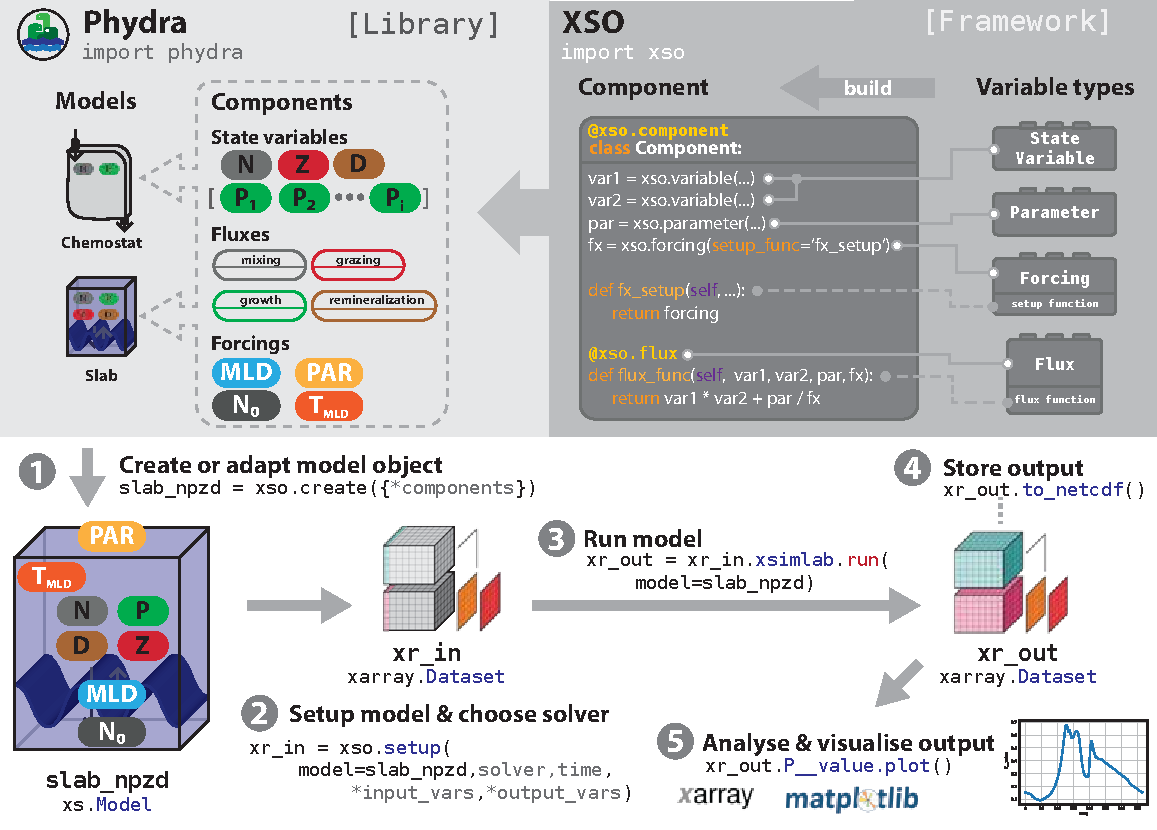
\includegraphics[width=12cm]{Figures/firstdraft_schematics/00_schematics_Package.pdf}
\caption{Schematic of package structure. Xarray-simlab-ode, an extension of Xarray-Simlab, provides the framework. Phydra is a library of functional components, that can be used, extended and modified. A typical workflow would consist of (1) Choosing a pre-existing model, modifying a model or creating a new model from components. (2) This model has to be setup with the correct labels and parameters, and a solver is chosen. (3) The model can be run efficiently, all input and output data is contained in Xarray datasets (4)  that can be conveniently stored or shared. (5) Model output can be conveniently analysed and visualized in the pre-existing scientific python ecosystem.}
\label{Figure:phydraschematics}
\end{figure*}

Phydra is a tool-box for marine ecosystem modeling, that is freely extensible by a user to be applied to many different use cases. Our goal is to make the technical implementation of writing functions and setting up a model more accessible, so that the focus can be on creating the most appropriate model structure and parameterisation for the specific scientific hypothesis that is being investigated. 

Constructing marine ecosystem models in Phydra is by design a flexible process, but the user can follow a general workflow of assembling models from the library of processes. This workflow is visualized in Figure \ref{Figure:phydraschematics} and will be further explained below.


\subsubsection{Model creation}

To create a Phydra model object, the desired processes defining state variables, forcings and fluxes have to be provided with their corresponding label to the \texttt{phydra.Model()} function.
The model can be assembled from the Phydra library, modifications of provided base classes or custom written processes. Multiple instances of fluxes or components can easily be added to the model, as long as the provided label differentiates them.
These labels will be the specific name of the process in this model instance. At model setup, the labels are used to reference a process and provide the appropriate parameters.

When creating a model, the xarray-simlab framework automatically checks that all references between processes are fulfilled, orders the processes in their logical order of execution and returns a Phydra model object. This model object contains all processes in the model and allows the user to view all parameters required as input at model setup. The Phydra library provides several basic model objects, that can be modified by a user through a simple interface that allows removing, modifying or adding new processes.

\subsubsection{Model setup}

A Phydra model object is itself only a collection of abstract processes. In order to fully initialize a model that can be solved, the model object needs to be supplied with a complete set of parameters.

This is done using the \texttt{phydra.create\_setup()} function. The necessary arguments to this function are the model object to be setup, all required input parameters, the time range to solve the model and the specific model output to save during runtime. The Phydra setup function is a thin wrapper around the Xarray-simlab model setup function that automatically includes the solver backend and clocks setup for the chosen solving method.

Phydra provides several options to store model output, as well as storing the value of fluxes and forcings. This allows users to specify the model output that suits the complexity of the model construct. There are processes supplied that can aggregate all state variables, Forcings or Fluxes values for output storage to simplify the process of defining output. For complex functional group models the output of each component can be stored along an individually labelled dimension, while a simple NPZD model can store the output of components along a shared dimension.

The function call returns an Xarray dataset object that contains all provided parameters as well as the initialized labelled model dimensions. This dataset can be passed with the appropriate model object to be solved in the next step, but also provides an interface to exchange parameters to easily modify an already instantiated model setup.

At model setup, the xarray-simlab framework supports batch dimensions of single or multiple parameters along which the model can be solved in parallel at runtime. This provides an efficient and intuitive interface to explore the parameter space of models.

\subsubsection{Runtime}
% -> model_instance.xsimlab.run()
% relatively straightforward, this will first initialize the model data variables according to the added processes and parameters supplied, and then start model evaluation
The model setup created in the previous step already contains the necessary parameters and labelled dataset for model runtime. All that is required of the user is to call the \texttt{xsimlab.run()} attribute and provide a model object that corresponds to the model setup. This does not have to be the same model instance used to create the setup, as long as specified parameters and output are compatible.

\textit{NOTE: Currently there is only one way to solve models in Phydra: using the GEKKO dynamic sequential solver (IMODE 7).. but there are a few options to relatively easily provide an interface for other types of solvers for future versions. Not sure if I should mention the following:}

-GEKKO provides a simple interface for steady state-simulations, and model optimisation. The models constructed with Phydra are completely compatible, simply the solver process needs to be exchanged (and for model optimisation an objective function needs to be defined additionally)

- GEKKO does as of yet not provide an adaptive step size solver like odeint, but I have created a feature request and talked to the developers. This will very likely be included in future versions.

\subsubsection{Model diagnostics and additional functionality}

- If the option is specified at setup, the model output will include not just the state variables, but the values of all fluxes. The magnitude of the fluxes can then easily be plotted...

- Xarray-simlab provides visualisation functions, that can be used to get a structured overview over all processes in a model instance. These are not optimized for the current structure though, as most dependencies between subprocesses are handled in the solver backend, not via explicit xarray-simlab process dependencies.

- Gekko stores model equations including the names of parameters and it would be possible to add some functions that print the mathematical equations.. which would be quite helpful to build and debug a model. (possible feature)

- Model optimisation (i.e. parameter fitting) is well supported by the GEKKO backend. I will run some tests, and if it works very well, it might make sense to include it in this publication, since it is a major strong point for using Phydra.


%% END OF SECTION 2
\clearpage



 %% \ SECTION 3
\section{Model use cases included with Phydra 0.1} \label{Section:UseCases}
% STAY AS FAR AS POSSIBLE AWAY FROM SPECIFIC PHYDRA/XARRAY_SIMLAB_ODE IMPLEMENTATION (I:E: LABELS ETC:) JUST TALK ABOUT COMPONENTS IF NECESSARY::

- included in first release are a collection of models and model components

To showcase the utility of Phydra, we present three model use cases of varying complexity. In this section, we present simplified descriptions of model structure and mechanisms, as well as parameterizations and model results. Per use case, we highlight a modification to the model that uses the functionality of the XSO framework.

- For Use Case 1 we will show full model setup, including variables, passing parameters, etc.
- The others will be presented more schematically, without complete mentions of all variables, but for all models full documented code is available, with exact code used for presented model runs and plots.

[This should be using the visualisation tool of xarray-simlab, that i need to modify to hide the backend of XSO (e.g. solver, etc.)]

- full model code, parameters, runs, code for plots etc. is available online for free
Additionally model and analysis code for all use cases is publicly available as documented interactive Jupyter notebooks in the Phydra repository (\url{https://github.com/ben1post/phydra/tree/master/examples}). 



\subsection{Model use case 1: Phytoplankton growth in a chemostat}
\begin{comment}
- IDEA: instead of Droop modification, run model at flow rate vs nut concentration grid and plot steady state biomass, then do same for periodic (mean nut vs flow rate) OR periodic mean vs amplitude = biomass OR 
- IDEA: can i use GEKKO optimization to match parameters for constant forcing, and then check if sinusoidal forcing deviates for the two different model formulations?
- IDEA: maybe remove the Sinusoidal Forcing bit? or focus on that instead of Droop? this double mod seems a bit complicated to present
\end{comment}

- Chemostats, a.k.a. continuous cultures, have been regularly used in exploring properties of phytoplankton! Seminal studies of Droop on nutrient uptake were performed using chemostats. \citep{Droop1968VitaminLutheri} 
- Very simple test-bed for more complex model setups (see Use Case 3)

- Here: Very simple model construct, phytoplankton growing on single nutrient, Monod uptake, linear flow rate
The simple model of \citet{Monod1942RecherchesBacteriennes}, devised to describe bacterial growth, assumes the growth rate is proportional to the nutrient uptake rate.

- first we check the model at constant flow rate and nutrient concentration, then (in order to show added value of framework) we add sinusoidal nutrient concentration and compare


In the following use case we will show the definition this models for growth of phytoplankton on a single nutrient in a chemostat environment. 
-The forcing will be both constant and sinusoidal


%%f
\begin{figure}[t]
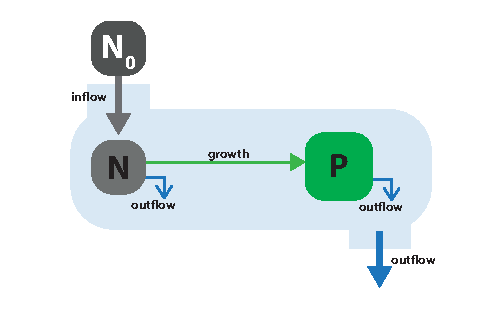
\includegraphics[width=8.3cm]{Figures/firstdraft_schematics/01_schematics_Chemostat.pdf}
\caption{Model schematic of chemostat model. Monod representation of phytoplankton feeding on a nutrient.}
\label{Figure:ModelSchematics_1}
\end{figure}

\subsubsection{Description}
The model is schematized in !Figure (a). It uses nitrogen as its currency (quantities are measured in units of $\mu mol$ N $m^{-3}$, or $\mu M$), with state variables for dissolved nutrients ($N$) and phytoplankton ($P$). The physical environment is a highly simplified flow-through system, corresponding to a laboratory chemostat setup. Growth medium with nutrient concentration $N_0$ flows into the system at rate $f$. The model components ($N$ \& $P$) flow out of the system at that same rate.

Nutrient limitation of phytoplankton growth ($\gamma$) is described via Monod kinetics \citep{Monod1942RecherchesBacteriennes}.
\begin{equation}
    \gamma = \frac{N}{k + N} 
\end{equation}
where $k$ is the half-saturation constant. $N$ is ambient nutrient concentration in the medium.
The realized growth rate is a product of the nutrient-limiting term $\gamma$ and the maximum growth rate $\mu^\emptyset$.
Pathways relating to detrital matter, mortality and regeneration are not resolved. 

The model equations are as follows:
\begin{equation}
    \frac{d N}{d t} = 
    f N^\emptyset % Nutrient mixing
    -  \mu^\emptyset \frac{N}{k + N} 
    - f N
\end{equation}

%PHYTOPLANKTON
\begin{equation}
    \frac{d P}{d t} =
    \mu^\emptyset \frac{N}{k + N} 
    - f P
\end{equation}

\subsubsection{Implementation}
% IDEA: instead of showing any code, show this also as a schematic (essentially the "map" of components and their variables) for the first simple example, I could show all steps of the process as well as the variables, etc. for the two more complex ones, I could isntead only show the name of the component in a box, and how they are interconnected (leaving out backend stuff)
The Monod model was implemented...

The above model can be separated into a few components:
State variables: N, P
Forcings: N0
Fluxes: Growth (N->P), Influx (N0->N), Outflux(N,P->)
This model can be implemented exactly like this in XSO, using 6 components. See the schematic (TODO!).

- Technical feature to explain: List-input for variable - used in Outflux component. It would be possible to add two model components for each variable that flows out, but tidier and more efficient to allow list input, Flux is computed in vectorized fashion in backend -> highly more efficient for many variables or larger dimensions.

- Parameters were chosen to represent a standard range, for specific applications and model to data comparisons these parameters should be checked again..

# table of parameters # here?

- In order to run this model at periodic forcing we can simply exchange the Forcing component, from ConstantForcing to SinusoidalForcing.


\subsubsection{Results}

- When run over a period of 10 days the model quickly reaches a steady state under constant forcing
- and shows an oscillating behaviour following the sinusoidal forcing 

- many more interesting checks and runs could be done, this is very simple example, and showcasing the ease of creating and modifying models using XSO and Phydra

%%f
\begin{figure}[t]
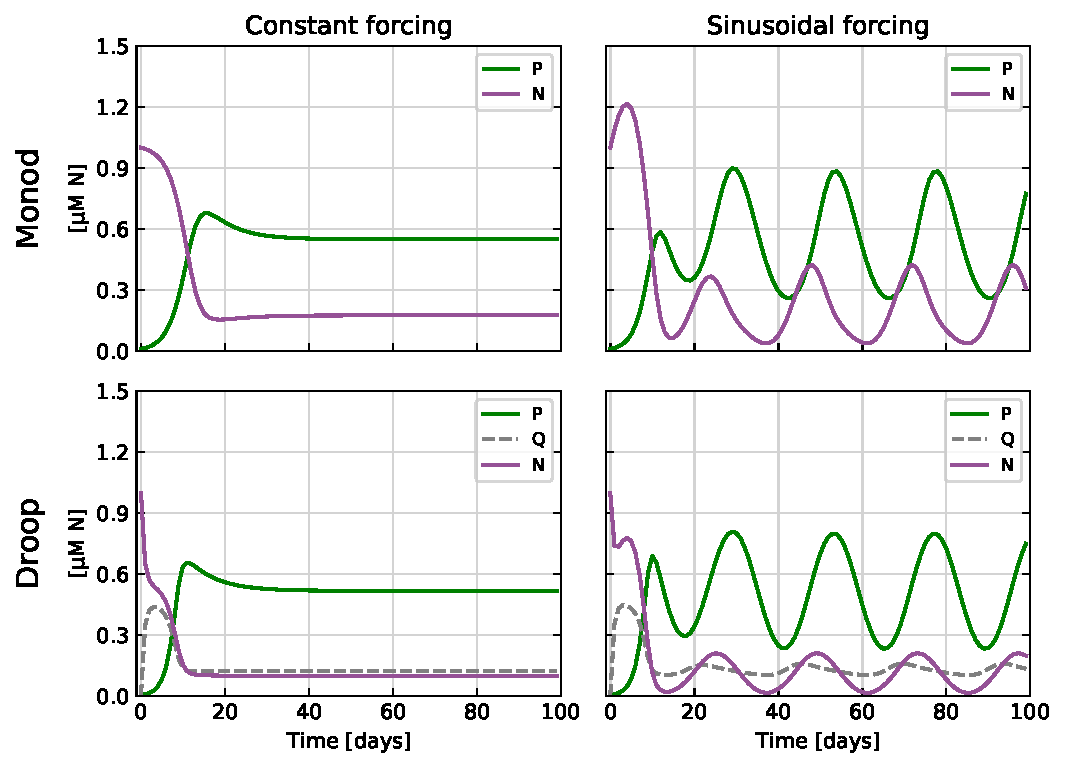
\includegraphics[width=8.3cm]{Figures/firstdraft_plots/01_chemostat_output.pdf}
\caption{Model output for the four chemostat model scenarios. (a) Monod - constant, (b) Monod - sinusoidal}
\label{Figure:ResultsChemostat}
\end{figure}


% NOTE: I DO NOT WANT A DISCUSSION HERE; BECAUSE THAT IS NOT THE POINT OF THE PAPER! IT SHOULD PRESENT TeCHNICAL FRAMEWORK AND IMPLEMENTATION; NOT DISCUSS MODEL Output.. still limitied discussion necessary in the "Result" sections per Use Case


\subsection{Model use case 2: An NPZD slab model - EMPOWER}
Our second use case presents a classical NPZD model embedded in a slab-ocean physical setting. The simplified two-layer structure provides a zero-dimensional and mechanistically simple description of physical processes affecting euphotic ecosystems in the open ocean. The classical structure lends itself well as an efficient physical test-bed for more complicated ecosystem descriptions and is often used as a teaching example.

The presented model is an implementation of the elegant EMPOWER model, as presented by \citet{Anderson2015c}. 
See Figure \ref{Figure:phydraschematics_1} (a) for a schematic of the model structure.

- Originally written in R as a script, modular structure achieved through hard-coded flags.
- We wanted to adapt the model to the flexible modular structure of XSO, very powerful test-bed for plankton modeling. That can also be used as a teaching tool and to explore formulations and parameters..

- Many different functions for different ecological processes exist, e.g. for light harvesting.
- Inspired by the comparison of light regimes in the original EMPOWER paper, we show how we rebuilt the model using XSO framework in Phydra. Now structure is modular, and does not require specific flags, can be used with many different solvers (no explicit for loop!) .. is it more efficient? (need to test!)
- Many other modifications are possible, and should be tested against different parameterizations.. ideally parameters grounded in physiology.


\subsubsection{Description}
% really present a concise and to the point model description here, as would be in any other model publication.
For the first use case we have implemented a traditional NPZD ecosystem model as presented in Figure \ref{Figure:phydraschematics_1} (a) with a nutrient $N$ (in this case nitrate), phytoplankton $P$, zooplankton $Z$ and detritus $D$ as state variables. The first use case model employs slab physics as presented in \citet{Evans1985ACycles}. The model ocean is built up of two layers. A biologically inert deep ocean is situated below a well mixed upper layer of variable depth that contains the ecosystem. The general model structure is adapted from the EMPOWER model presented by \citet{Anderson2015c}.
Modifications were aimed at simplifying the description of physical forcings and phytoplankton growth. The model is driven by empirical forcing describing the depth of the mixed layer ($H$), average temperature of the mixed layer ($T$), photosynthetically active radiation at the surface ($I$) and nutrient concentration in the deep layer ($N^\emptyset$) 

% Nutrient dynamics
The zero-dimensional physical slab setting describes two vertical layers of which the deeper layer supplies nutrients to the upper layer, whilst other components are mixed to the deep layer and lost from the system.
The magnitude of mixing is described by the coefficient $K$:

\begin{equation}
    K = \frac{h^{+} + \kappa}{H}
\end{equation}

Constant diffusive mixing is parameterized by $\kappa$. Variable mixing is a function of the change in MLD over time $h = \frac{d}{d t} H$. The derivative of MLD ($h$) is positive when the mixed layer deepens. The function $h^{+}$ defines the effects of entrainment and detrainment due to the changes in MLD as $h^{+} = \max(0, \ h)$. When the mixed layer shallows, $h^{+}$ does not modify $K$ (i.e. returns 0 instead of a negative value), based on the assumption that detrainment of mass and the increase in concentration due to the reduced volume of the mixed layer are balanced \citep{Evans1985ACycles}. 

%\subsubsection{Nutrients}
Dissolved inorganic nitrogen in the mixed layer ($N$) is supplied via mixing, zooplankton excretion and detritus remineralisation.
Nutrients are entrained from the bottom layer. Mixing of nutrients is a positive term adding to $N$ along the gradient between $N^\emptyset$ and $N$. The general direction of transport is from a nutrient-rich bottom layer to the upper layer supporting phytoplankton growth, which is the only loss term.

%\subsubsection{Phytoplankton}
Phytoplankton biomass ($P$) increases through temperature-dependent, light- \& nutrient-limited growth. The growth rate ($\mu^{P}$) is the product of a maximum growth rate ($\mu^{\emptyset}$) and the growth-dependencies on temperature ($\gamma^{T}$), light ($\gamma^{I}$) and nutrients ($\gamma^{N}$): 

\begin{equation}
    \mu^{P} = \mu^{\emptyset} \ \gamma^{T} \ \gamma^{I} \ \gamma^{N}
\end{equation}

$T$ is the average temperature of the mixed layer in \unit{\degree C}, as supplied from model forcing. Temperature dependence of the growth rate ($\gamma^{T}$) is calculated via the Eppley curve \citep{Eppley1972TemperatureSea}, with an exponential equivalent to a $Q_{10}$ of 1.895.

\begin{equation}
    \gamma^{T} = \exp{(0.063 \ T)} \label{mumax}
\end{equation}

The light-limiting term $\gamma^{I}$ represents growth-dependence on total light ($I$) available to phytoplankton the upper mixed layer. We use a simplified form of Steele's formulation to describe light-limitation of phytoplankton growth in the mixed layer, as adapted from \citet{Acevedo-Trejos2016} and originally described in \citet{Steele1962EnvironmentalSea}.

\begin{equation}
    \gamma^{I} = \frac{1}{H} \int_{0}^{H}\left[ \frac{I(z)}{I^{opt}} \cdot \exp{\left( 1 - \frac{I(z)}{I^{opt}} \right) }  \right]dz \label{steele1}
\end{equation}

Where $I^{opt}$ is the light level at which photosynthesis saturates and $I(z)$ is the irradiance at depth $z$.
The irradiance forcing $I$ is a temporally and spatially averaged monthly climatology of photosynthetically active radiation (PAR) at the surface. 

Attenuation of $I$ at depth $z$ in the mixed layer is calculated according to the Lambert-Beer equation:

\begin{equation}
    I(z) = I \ \exp{(-k^{PAR} \ z)} \label{beer}
\end{equation}

The attenuation coefficient $k^{PAR}$ is the sum of the attenuation coefficient of seawater $k^w$ and that of phytoplankton biomass $k^c$, which is multiplied by the current phytoplankton biomass $P$:

\begin{equation}
    k^{PAR} = k^w + k^c \cdot P
\end{equation}

Combining the equations and integrating across the mixed layer, the numerical solution for the integrated light-limiting term affecting phytoplankton growth is calculated. Integrated values within the mixed layer larger than the optimal irradiance will limit growth, to model effects of photo-inhibition \citep{Steele1962EnvironmentalSea}.

$$ALSO! SHOW 3-layer MLD! explain and show equations$$ *here #TODO

This simple implementation uses only one parameter to describe light limitation of phytoplankton growth, which is $I^{opt}$. This is a highly simplified treatment of light in a slab model. A more realistic representation of light-limited growth would include chlorophyll-to-biomass ratios and related parameters and functions. See \citet{Anderson2015c} for an insightful discussion of light-limitation in slab models.

Nutrient limitation of phytoplankton growth $\gamma^N$ is described by the Michaelis-Menten (or Monod) equation.

\begin{equation}
    \gamma^N = \frac{N}{k^N + N}
\end{equation}

where $k^N$ is the half-saturation constant for nutrient uptake. $N$ is the ambient nutrient concentration, in this case of dissolved inorganic nitrogen (DIN). In this simple model there is no distinction between nutrient uptake and assimilation of nutrient via growth.

Non-grazing mortality of phytoplankton is described by both a linear $m^P$ and a quadratic factor $m^{P2}$ \citep{Yool2011Medusa-1.0:Domain}. The former accounts for natural mortality and excretion. Quadratic mortality describes density-dependent loss processes, which can be caused by viral infection. All non-grazing loss terms feed into the detritus pool.

%\subsubsection{Zooplankton}
Grazing by zooplankton occurs on both phytoplankton and detritus. The grazing function is a Holling Type 3 grazing response as presented in \citet{Anderson2015c}:

\begin{equation}
    G^P = \mu^Z \left( \frac{ \hat{\phi}^P P}{(k^Z)^2 + \hat{\phi}^D D +\hat{\phi}^P P}  \right) Z
\end{equation}
where $\hat{\phi}^P$ = $\phi^P \ P$, $\hat{\phi}^D$ = $\phi^D \ D$.

This formulation describes the total biomass of phytoplankton that is grazed $G^P$. Parameter $\mu^Z$ is the maximum ingestion rate for a food source, in this case both phytoplankton and detritus. 
The grazing preference parameters $\phi^P$ and $\phi^D$ do not represent a discrete fraction of the amount grazed in the diet relative to the environment. Instead, this amount is represented by the ratio of $\hat{\phi}^P$ and $\hat{\phi}^D$. 
The half-saturation constant for grazing $k^Z$ is similarly an arbitrary parameter, that scales the density-dependent half-saturation constant $k^P$ for grazing on phytoplankton based on the choice of $\phi^P$, with the relationship $k^P$ = $\sqrt{\frac{(k^Z)^2 }{ \phi^P}}$.


Similarly the detritus grazing flux is defined as:

\begin{equation}
    G^D = \mu^Z \left( \frac{ \hat{\phi}^D D}{(k^Z)^2 + \hat{\phi}^D D +\hat{\phi}^P P}  \right) Z
\end{equation}

This sigmoidal response includes passive prey switching via an interference effect, where the increase in biomass of one prey slightly reduces the intake of other prey. In contrast to other grazing formulations \citep[e.g.][]{Fasham1990a}, the prey switching mechanism does not create sub-optimal feeding, where an increase in biomass of less common prey can decreases the total grazing flux \citep{Gentleman2003a}.

Zooplankton ingestion of prey does not directly convert to biomass gained however. The total biomass grazed ($G^P + G^D$) is split three ways between zooplankton growth (to $Z$), excretion of dissolved nutrients (to $N$) and egestion of faecal matter \& particles (to $D$). Zooplankton growth is a product of total biomass grazed ($G^P$) and the gross growth efficiency (GGE) of zooplankton. The two parameters defining GGE in this model are absorption efficiency ($\beta$) and net production efficiency ($\epsilon$). Adsorption efficiency $\beta$ describes the fraction of $G^P$ which is absorbed in the gut, of which the fraction $\epsilon$ is actually assimilated into biomass (to $Z$: \ $\beta \epsilon$), while the rest is excreted as DIN (to $N$: \ $\beta (1-\epsilon)$). GGE specifically is the product of $\epsilon$ and $\beta$, for which values between 0.2 and 0.3 have been observed for a wide range of zooplankton \citep{Straile1997GrossGroup}. The fraction of $G^P$ egested to $D$ (e.g. as faecal pellets) is calculated via $1-\beta$. 

Similar to phytoplankton mortality, the linear mortality factor $m^Z$ parameterizes natural mortality and excretion and feeds into the pool of detritus. The quadratic factor $m^{Z2}$ describes higher order predation on zooplankton and is removed from the system. 


%\subsubsection{Detritus}
Detritus concentration in the upper layer ($D$) is supplied by all mortality of phytoplankton, linear zooplankton mortality and zooplankton egestion (e.g. faecal pellets). The loss terms are remineralisation, zooplankton grazing, mixing and an additional sinking flux. 

Detritus is remineralised at a constant rate $m^D$. Similar to $P$ and $Z$, $D$ is affected by mixing through changes in MLD, described by the mixing coefficient $K$. In addition to $K$, detritus experiences losses due to gravitational sinking at a rate of $v^D$. This term is added to describe the fast export of larger detritus particles below the mixed layer. 

%\subsubsection{Model equations}
The rates of change of the state variables are described by the following set of equations. For the definition of all symbols used here see Table \ref{appendix:table:usecase1symbols}. See \citet{Anderson2015c} for a more detailed discussion of model structure and formulation.

\begin{equation}
    \frac{d N}{d t} = 
    K (N^\emptyset - N) % Nutrient mixing
    + \beta(1 - \epsilon)(G^P + G^D) % Unassimilated grazing by Z
    + m^D \ D % Remineralisation of D
    - \mu^{P} \ P % Phytoplankton gains
\end{equation}

%PHYTOPLANKTON
\begin{equation}
    \frac{d P}{d t} =
    \mu^{P} \ P  % Phytoplankton gains
    - m^P \ P % Linear mortality
    - m^{P2} \ (P)^2 % Quadratic mortality
    - G^P % Z grazing
    - K \ P % Phytoplankton mixing
\end{equation}

%ZOOPLANKTON
\begin{equation}
    \frac{d Z}{d t} =
    \beta \ \epsilon(G^P + G^D) % Assimilated grazing
    - m^Z \ Z % Linear mortality
    - m^{Z2} \ (Z)^2 % Quadratic mortality
    - K \ Z % Zooplankton mixing
\end{equation}

%DETRITUS
\begin{equation}
    \frac{d D}{d t} = 
    m^P \ P % Linear mortality
    + m^{P2} \ (P)^2 % Quadratic mortality
    + m^Z \ Z % Linear mortality
    + (1 - \beta)(G^P + G^D) % Unassimilated grazing by Z
    - G^D % Z grazing on D
    - m^D \ D % Remineralisation of D
    - K \ D % Mixing of D
    - \frac{v^D}{H} \ D % Sinking of D
\end{equation}


%%f
\begin{figure}[t]
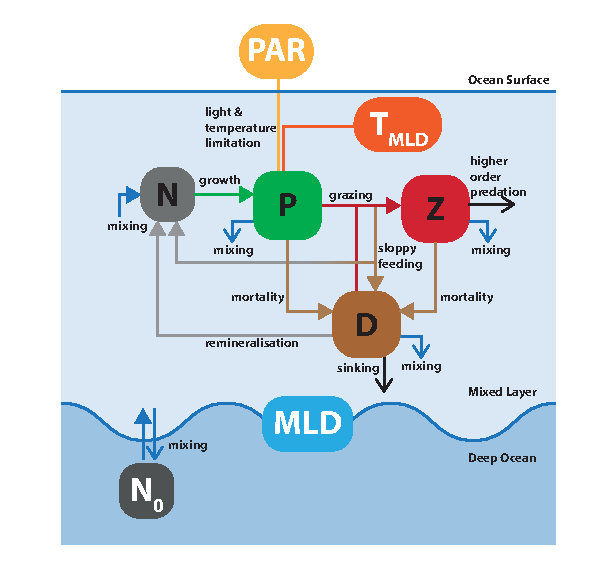
\includegraphics[width=8.3cm]{Figures/firstdraft_schematics/02_schematics_EMPOWER.pdf}
\caption{Model schematic of NPZD slab model for example 1. Model structure and parameterisation is adapted
from \citet{Anderson2015c}}
\label{Figure:ModelSchematics_2}
\end{figure}


%% HERE SLAB OUTPUT

\subsubsection{Implementation}
% here present the implementation as is used in phydra
% IDEA: instead of showing any code, show this also as a schematic (essentially the "map" of components and their variables) for the first simple example, I could show all steps of the process as well as the variables, etc. for the two more complex ones, I could isntead only show the name of the component in a box, and how they are interconnected (leaving out backend stuff)
The model was implemented as follows...
(- more simplified description of model, less detailed schematics due to size contraints)

- we followed EMPOWER model structure, but technical implementation using XSO is quite different: we modified the explicit time-step (in a for-loop) scheme to fully integrated functions, that can be computed irrespective of time step size. This makes the functions and code easier to read and modify.
- Model code is not directly tied to integration or time-step scheme, everything flexible!


$$HERE$$ need to edit this to large table, for all models $$HERE$$
The above model can be separated into a few components:
State variables: N, P, D, Z
Forcings: N0, SST, MLD, Temp, I0(calculated from location)
Fluxes: Uptake (N->P), Growth (P->Z,N,D GGE), Upwelling (N0-MLD>N), Mixing(N,P,Z->),..
This model can be implemented exactly like this in XSO, using X components. See the schematic (TODO!).

- Schematic of implementation is only shown simplified here, but full description and code available online! (and appendix?)

- more complex model requires using features of XSO to have efficient code, e.g. one component calculating K, which is used in Mixing & Upwelling component. Also there is growth limitation, which is a multiplicative process of a few different factors (That are the results of "fluxes"). This can both be done using the $group$ variable type. EXPLAIN IT, Can have multiple levels, e.g. for temperature dependency here (could also have this in same process though!)

- Again, use some list-input Variables. EXPLAIN GGE routing, and why it is done that way

- Grazing function, allows for list input! Can vary and experiment with what Zooplankton grazes on. Implementation relatively simple because Z has no dimensions.

- Complex calculation of light, via latitude. NOwadays also robust data from Satellite (which is already integrated climatology).. with modular structure complexity can easily be removed and other simpler forcing provided.. or light forcing can be calculated outside of model, and then passed to model fully integrated (this is what Phydra does) -> more efficient.

- parameters are completely adapted from Anderson et al.
* Table of Parameters here *
- four locations from original paper are adapted, exact same forcing is used (see forcing figure!)
- Verification data is different from original paper, chlorophyll MODIS climatology and WOA 2018 nutrient data (Nitrogen) + MLD climatology.

- showcase "batch" execution, can run all 4 location models in parallel. Output is stored as one Xarray, with additional dimension coordinate that differentiates between locations..


% DO I NEED A NEW SUBSECTION FOR FORCING? HOW TO DO THIS?
%%f
\begin{figure*}[t]
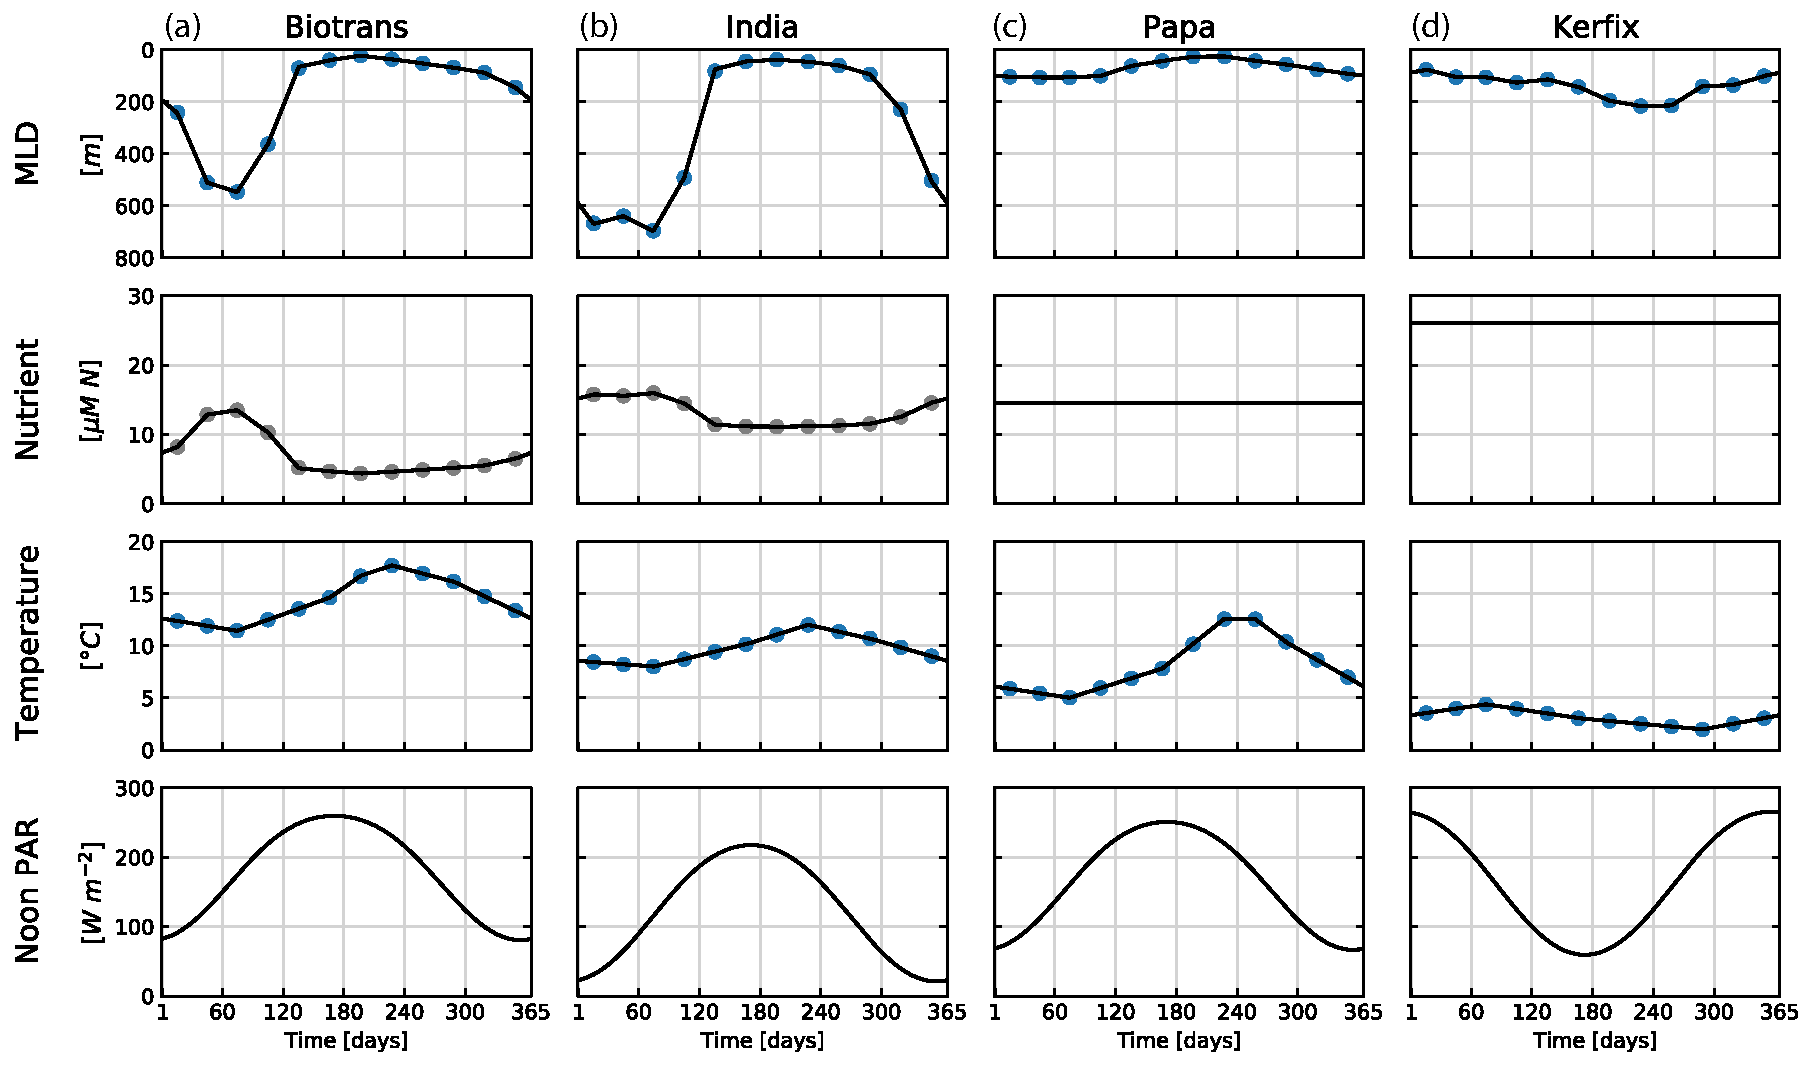
\includegraphics[width=15cm]{Figures/firstdraft_plots/02_EMPOWER_forcing.pdf}
\caption{Forcing is shown for the four locations: Mixed Layer Depth (MLD), Nitrate below the Mixed Layer ($N_0$), Photosynthetically Active Radiation (PAR) and temperature averaged across the Mixed Layer ($T_{MLD}$). Mixed layer depth and temperature data from Anderson et al. 2015. Nutrient forcing is a function of depth for locations Biotrans and India, and a constant value for Papa and Kerfix. Irradiance is calculated as a function of latitude.}
\label{Figure:EMPOWERforcing}
\end{figure*}


- modification:

- Calculating light avaiability via Lambert-Beer for a single layer (MLD) is very rough approximation
- Slab model is already strong simplification of ocean, but even within MLD light is attenuated quite differently. EMPOWER paper has an interesting discussion of this, and shows more complex treatments.
- We have implemented one of the described formualtions: a three-layer MLD for light attenuation, 0-5, 5-25, >25 meters
- can be even more complex, such as the described formulations treating spearate spectral bands.
- decision of modeler how complex, how simple, depends on scientific question & location of model




\subsubsection{Results}
% show model results and discuss 
- Recreating results of EMPOWER paper with our framework
- Different integration routines, but output in high agreement (This should never change the model output!)
- Different verification data, but generally same pattern, and agreeing well 

- showing different light integration routine: as observed in EMPOWER, 3-layer light attenuation shows model results closer to data, particularly in location Papa



%% HERE SLAB OUTPUT
%%f
\begin{figure*}[t]
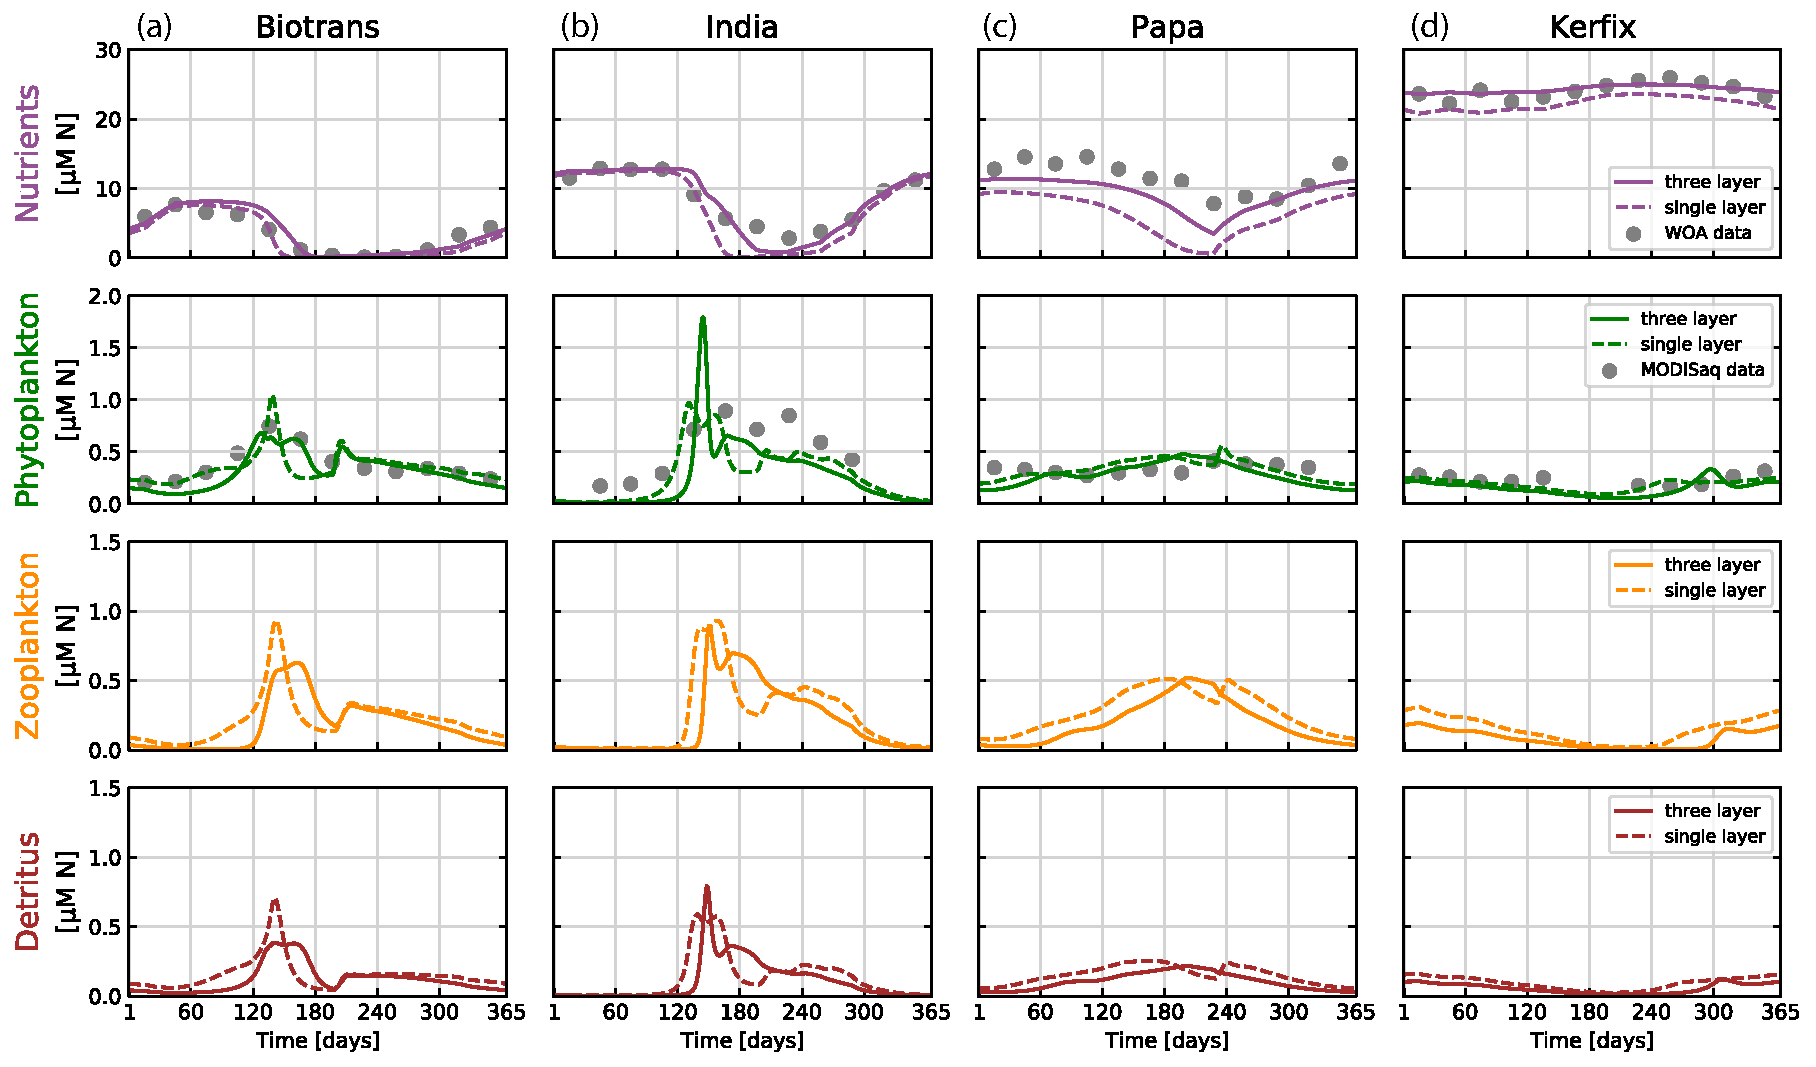
\includegraphics[width=15cm]{Figures/firstdraft_plots/02_EMPOWER_lightcomp.pdf}
\caption{Comparative slab model runs, EMPOWER model locations and forcing. Three layer model of light attenuation in the mixed layer is thick line. Single layer model is dashed line. Verification data for Nitrogen in the upper mixed layer is taken from WOA 2018. Phytoplankton verification data is monthly climatology derived from MODIS aqua observations, C-to-Chlorophyll ratio of 75 is assumed in model and used to calculate conversion, in addition to a Redfield ratio of 16:1 for C-to-N.}
\label{Figure:ResultsEMPOWER}
\end{figure*}



\subsection{Model use case 3: A complex size-based NPZ model - ASTroCAT}

From an attempt at describing an oceanic physical setting with a highly simplified ecosystem, we move to a simplified laboratory setting with a complex description of a size-structured ecosystem. The model structure for the second use case was adapted from \cite{Banas2011b}. See Figure \ref{Figure:phydraschematics_1} for a schematic of the model structure. 

- Banas publication features extended investigation of model dynamics, also under variable forcing, and stochastic grazing, etc. but here we focus on the simplest setup under constant forcing.
- simple box model, many processes not resolved


- allometric phytoplankton growth and zooplankton grazing, one level of trophic interaction highly resolved
Size is called a "master-trait" in the trait-based description of plankton ecology, allowing modellers and ecologist to describe the diverse plankton community along one continuous axis. (This is of course an oversimplification, and it takes careful consideration of the choice of allometries and often a combination of functional properties and size classes to achieve a more realistic representation of natural phytoplankton assemblages.)

- results in system with emergent properties

- XSO framework, allows adding dimensions to state variables, has (Numpy) vectorization capabilities built in, the model can be initialized with a flexible number of size classes of phytoplankton and zooplankton (always equal number though, for this model)

- We showcase this feature by running the model with 2 to 50 clones and comparing bulk phytoplankton biomass between runs



\subsubsection{Description}
% really present a concise and to the point model description here, as would be in any other model publication.

For the second use case we have implemented a size-spectral NPZ ecosystem model as presented in Figure \ref{Figure:phydraschematics_1} (b) with a nutrient $N$ (in this case nitrate), multiple size classes of both phytoplankton $P_i$ and zooplankton $Z_j$ as state variables. 
This model use case employs a simple chemostat as physical setting. A flow-through culture, where organisms grow in a bottle with a continuous influx of a nutrient solution. At the same rate all components of the bottle flow out of the system, so that volume remains constant over time.
Model structure and parameterisation is adapted from the ASTroCAT model \citep{Banas2011b}, with slight modifications to the physical environment and parameterisation. 

The model describes a size-structured community of phytoplankton and zooplankton, with each state variable defined by their equivalent spherical diameter (ESD). In model runs presented in this paper, we follow \citet{Banas2011b} in running simulations with 40 size classes of equally log-spaced ESD of $P$ (1 to 20 \unit{\mu m}), and 40 matching classes of $Z$ (2.1 to 460  \unit{\mu m}). 
The model can be defined with any number of size classes within meaningful boundaries of the allometric parameterisation. Size classes are denoted by the subscript $i$ for phytoplankton and $j$ for zooplankton. In the implementation of a size-spectral model by \citeauthor{Banas2011b} the food-web is implicitly made up of matching pairs of $P_i$ and $Z_j$, to avoid creating classes at the ends of the size spectrum that are artificially released or suppressed by grazing pressure.

%\subsubsection{Nutrient}
Dissolved inorganic nitrogen (DIN) in the model system ($N$) is supplied from influx of medium (with nutrient concentration $N^\emptyset$) at a constant rate $f$ and the fraction of grazed biomass that is excreted by $Z$. The concentration $N^\emptyset$ and the flow rate $f$ determine the total nutrient supply to the system. At the same rate $N$ is flowing out from the system. Zooplankton excretion is a recycled term, that also adds back into the pool of $N$. The major loss term to $N$ is phytoplankton growth.

%\subsubsection{Phytoplankton}
Phytoplankton biomass $P$ increases through  nutrient-limited growth. Nutrient limitation of phytoplankton growth $\gamma_i^N$ is described by the Michaelis-Menten (or Monod) equation:

\begin{equation}
    \gamma_i^N =  \frac{N}{k_i^N + N} 
\end{equation}

where $k_i^N$ is the size-dependent half-saturation constant. $N$ is ambient nutrient concentration in the medium.

Non-grazing mortality of phytoplankton is described the factor $m^P$ that is scaled by the maximum intrinsic growth rate $\mu_i^{\emptyset}$. This accounts for natural mortality and excretion.

%\subsubsection{Zooplankton}
Zooplankton size class $j$ grazing on phytoplankton size class $i$ is calculated by
\begin{equation}
    G_{ij}^P = \mu_j^Z \ \frac{ \phi_{ij} \cdot P_i }{ k_j^Z + \sum_{i}(\phi_{ij} \cdot P_i) } \ Z_j
\end{equation}
where $\mu_j^Z$ is the size-dependent maximum ingestion rate, $k_j^Z$ is the prey half-saturation level and $\phi_{ij}$ is the relative preference of $Z_j$ for prey type $P_i$.

Prey preference is assumed to vary with phytoplankton size $size_i^{P}$ in a log-Gaussian distribution around an optimal prey size for each grazer $size_j^{opt}$.

\begin{equation}
    \phi_{ij} = exp \left[ -\left( \ \frac{ log_{10}(size_i^{P}) - log_{10}(size_j^{opt}) }{ \Delta size^{P} } \right) \right]
\end{equation}
Where $\Delta size^{P}$ is the prey size tolerance parameter, with units of \unit{log_{10}(\mu m)}, that controls the width of the Gaussian distribution.

Zooplankton growth is a product of total biomass grazed ($G^P$) and the gross growth efficiency (GGE) of zooplankton. The two parameters defining GGE in this model are absorption efficiency ($\beta$) and net production efficiency ($\epsilon$). Adsorption efficiency $\beta$ describes the fraction of $G^P$ which is absorbed in the gut, of which the fraction $\epsilon$ is actually assimilated into biomass (to $Z$: \ $\beta \epsilon$), while the rest is excreted as DIN (to $N$: \ $\beta (1-\epsilon)$). GGE specifically is the product of $\beta$ and $\epsilon$, for which values between 0.2 and 0.3 have been observed for a wide range of zooplankton  \citep{Straile1997GrossGroup}. The fraction of $G^P$ egested (e.g. as faecal pellets) is calculated via $1-\beta$, which in the current model setup is assumed to be exported quickly in the flow-through setting and lost from the system. 

Zooplankton experiences quadratic mortality according to the parameter $m^{Z2}$, describing higher-order mortality and predation of zooplankton that is removed from the system \citep{Edwards2000TheModels}. This closure term is quadratic, calculated with the implicit assumption that mortality of $Z_j$ is proportional to total zooplankton biomass $\sum_{j} Z_j$.


%\subsubsection{Model equations}
The rates of change of the state variables are described by the following set of equations. See \citet{Banas2011b} for a more detailed discussion of model structure and formulation.

\begin{equation}
    \frac{d N}{d t} = 
    f \ N^\emptyset % Nutrient mixing
    +  \beta (1 - \epsilon) \sum_{j} \sum_{i} G_{ij}^P % Unassimilated grazing by Z
    - \sum_{i} ( \mu_i^{\emptyset} \ \gamma_i^N \ P_i) % Phytoplankton gains
\end{equation}

%PHYTOPLANKTON
\begin{equation}
    \frac{d P_i}{d t} =
    \mu_i^{\emptyset} \  \gamma_i^N \   P_i  % Phytoplankton gains
    - m^P  \ \mu_i^{\emptyset} \ P_i % Linear mortality
    - \sum_{j} G_{ij}^P % Z grazing
\end{equation}

%ZOOPLANKTON
\begin{equation}
    \frac{d Z_j}{d t} =
    \beta \ \epsilon \ \sum_{i} G_{ij}^P % Assimilated grazing
    - m^{Z2} \ Z_j \ \sum_{j} Z_j  % Quadratic mortality
\end{equation}



\begin{table*}[t]
\caption{Allometric parameterisations and empirical parameter values employed in use case 2, adapted from \citet{Banas2011b}.}
\begin{tabular}{l l l l l}
Empirical fit & Applicability & Source \\
\tophline
$\mu_i^{\emptyset} = (2.6 \ d^{-1}) \left( \frac{size_i^{P}}{1\mu m} \right)^{-0.45}$ & Phytoplankton 1-100 ESD \unit{\mu m} & Tang(1995) \\
$k_i^N = (0.1 \ \unit{µM \ N})\left( \frac{size_i^{P}}{1\mu m} \right)$ & Phytoplankton 1-100 ESD \unit{\mu m} & Eppley et al. (1969) \\

$\mu_j^Z = (26 \ d^{-1})\left( \frac{size^i_{P}}{1\mu m} \right)^{-0.4}$ & Flagellates, dinoflagellates, ciliates, copepods & Hansen et al. (1997) \\

$k_j^Z = 3 \ \unit{µM \ N} $ & Flagellates, dinoflagellates, ciliates, copepods & Hansen et al. (1997) \\

$size_j^{opt} = (0.65 \ \unit{\mu m})\left( \frac{size^i_{P}}{1\mu m} \right)^{0.56}$ & Flagellates, dinoflagellates, ciliates, copepods & Hansen et al. (1994) \\
$\Delta size^{P} = 0.25 $ & Ciliates, nauplii, copepodites & Hansen et al. (1994)  \\
\middlehline

\bottomhline
\end{tabular}
\belowtable{TODO: the sources need to be added properly! for now just text..} % Table Footnotes
%\label{appendix:table:usecase2parameters}
\end{table*}
%

%%f
\begin{figure}[t]
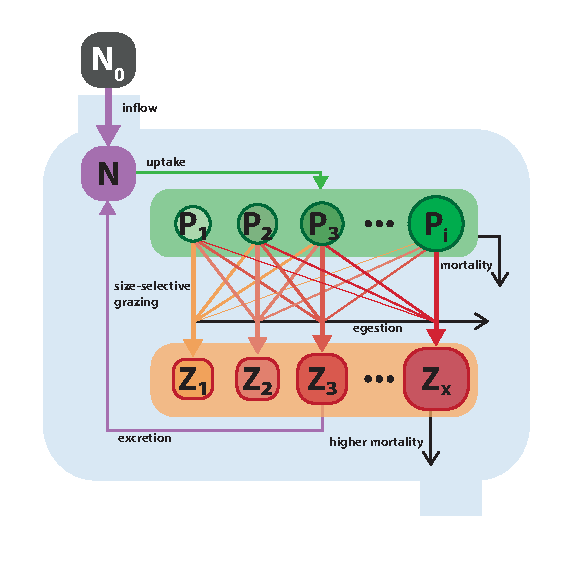
\includegraphics[width=8.3cm]{Figures/firstdraft_schematics/03_schematics_ASTroCAT.pdf}
\caption{Model schematic of size-structured $NP_{40}Z_{40}$ trophic model. Model structure and parameterisation is adapted from \citet{Banas2011b}.}
\label{Figure:ModelSchematics_3}
\end{figure}

\subsubsection{Implementation}
% here present the implementation as is used in phydra
Implementation is similar to Banas, but in Python, not Javascript/Processing. Model structure exactly the same.
Using XSO framework we don't need to use any for-loops, can make use of vectorization.


$$HERE$$ need to edit this to large table, for all models $$HERE$$
The above model can be separated into a few components:
State variables: N, P, Z
Forcings: N0 (very easy to go from constant to sinusoidal forcing)
Fluxes: Uptake (N->Pp), Grazing (Pp->Zz + GGE->N,loss), Influx (N0->N)
This model can be implemented exactly like this in XSO, using X components. See the schematic (TODO!).

- Schematic of implementation is only shown simplified here, but full description and code available online! (and appendix?)

- SV-Array functionality! Dimensionality of state variables (this functionality in XSO) is useful is in setting up phytoplankton size classes in trait-based models. All phytoplankton state variables grow on a common nutrient, but uptake parameters are related to allometries of cell size. A phytoplankton functional group is initialized, with a certain size range and number of state variables. Parameters are dynamically initialized based on the size provided by the component. 

- Allometries are not built into model, to reduce complexity and increase flexibility.. instead they are provided as helper functions with Phydra -> can be used for any project! What is input variable in model is not size but the actual parameter. Model however does store the size variable, as this is required input for the Size-based SV component (additional param). This way users can store any necessary information with model data.. (this should also be xs.index, helps with plotting (TODO))

- E.g. for mortality, intuitive writing of flux functions, because of vectorization: sum of Z can be computed against each Z, array is returned from function

- Implementation of Grazing function is very complex, as many size classes create large complex matrix-wise interaction. With XSO computational optimization, we use vectorization again, and multi-dimensional flux! Works without problems, but need to keep attention to orientation and correct parsing of matrix (Could provide helper functions? -> think about it)

- modification: very simple! use SV-Array component, and provide variable number of initial values in list, model automatically scales all other functions etc.


\subsubsection{Results}
- recreate dynamics observed using the same model by BANAS
- showing oscillatory behaviour, emergent properties of complex food web (one level of trophic interaction)
- modification: interesting effect of the number of size classes on model output and model stability.. seems to stabilize (but still vary) after 10-20 clones -> important fact for functional group type models! dynamics are an artifact of low resolution, not functional diversity. With increased resolution, more "predicatable" dynamics.


%%f
\begin{figure}[t]
\includegraphics[width=8.3cm]{Figures/firstdraft_plots/03_ASTroCAT_N50P50Z.pdf}
\caption{Nutrient concentration and biomass under steady nutrient forcing in model run resolving 50 size classes. Size classes are log-spaced in a range of 1 to 20 and 2.16 to 420. (a) Nutrient concentration over time. (b) Phytoplankton biomass by size class over 10 years of model time evolution. (c) Zooplankton time evolution over the same period.}
\label{Figure:ResultsASTroCAT_1}
\end{figure}


%%f
\begin{figure}[t]
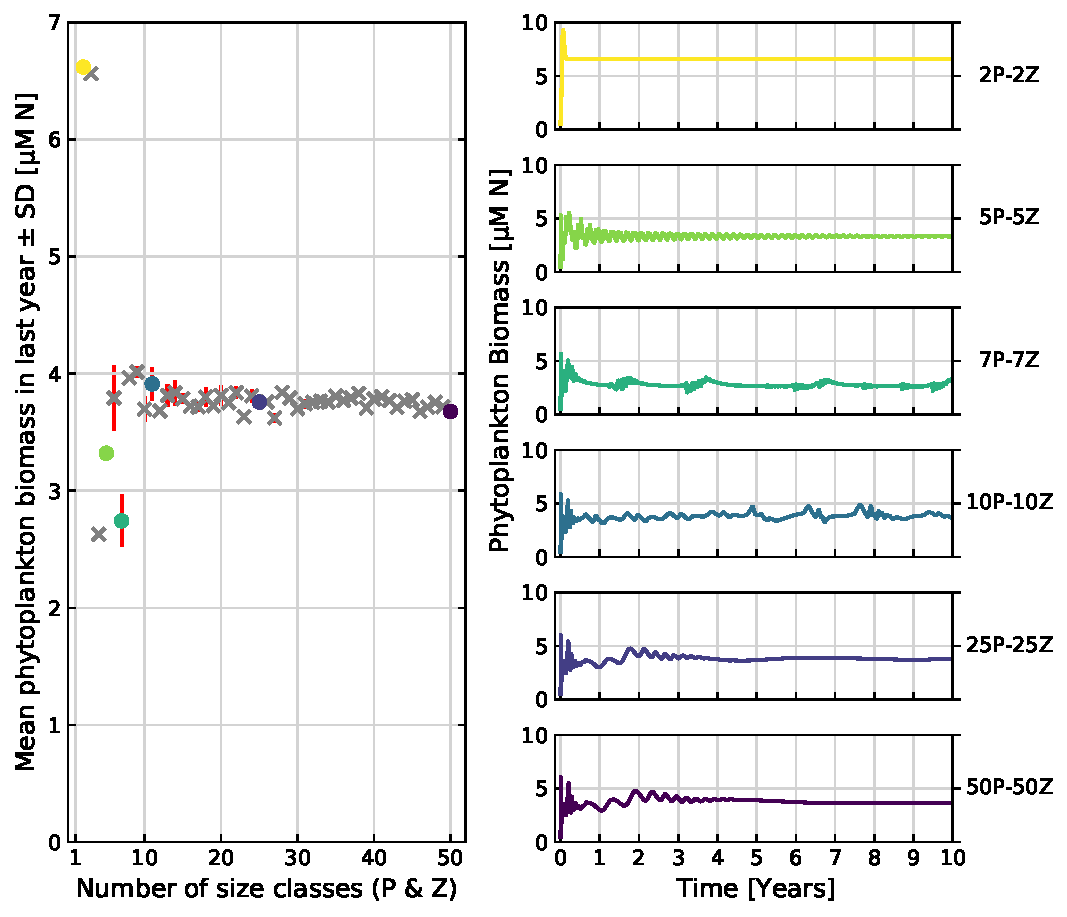
\includegraphics[width=8.3cm]{Figures/firstdraft_plots/03_ASTroCAT_sizeclassrange.pdf}
\caption{Comparative runs of varying number of size-classes. (a) Mean biomass of phytoplankton over the last year of a ten year run over a range of 2 to 50 size-classes of Phytoplankton and Zooplankton. Standard deviation is plotted in red. Grey crosses mark runs not otherwise shown, colored dots correspond to exemplary runs. (b) Exemplary model runs. Sum of phytoplankton biomass is shown over a ten year run.}
\label{Figure:ResultsASTroCAT_2}
\end{figure}


%%% added Section for editing purposes, later simply use \conclusions
\section{Conclusions}
\conclusions  %% \conclusions[modified heading if necessary]
% Place this project in the wider open science ecosystem, outlook on further developments

% ANDREWS COMMENTS
make the main points again (from intro)
old school modeling can be done better
show that I am moving in a direction that other people are! Brian Rose climlab, etc.

- This is a first step in the direction

- package architecture should be merged with other open-source python efforts (veros-bgcm, BGC-val)

- xsimlab is a powerful framework that is actively developed further, more added compatibilities possible
- same goes for xarray-simlab-ode, e.g. solvers, visualization, optimization of model construction & execution in backend

e.g. next steps: 1. add 1D, 2D, 3D models 2. add agent-based models using xarray-simlab framework (could use the same pool of functions, compability could be established with backend code!)

- Python lends itself well to interface with legacy fortran code, can make marine 3d modeling much more accessible without loosing performance or accuracy

- want to make the first step, hoping that people will adopt and contribute

- any modeler willing to use phydra will probably have to write his own processes, and this is also the intention. Object oriented structure still highly simplifies collaboration with non-modelers or people not versed in higher-level python. Higher transparency and collaboration between modelers as well, since same code base and similar 

- clearly: should add 1D -> 3D example models in the future


%% END OF SECTION CONCLUSIONS









%% The following commands are for the statements about the availability of data sets and/or software code corresponding to the manuscript.
%% It is strongly recommended to make use of these sections in case data sets and/or software code have been part of your research the article is based on.

\codeavailability{TEXT} %% use this section when having only software code available


\dataavailability{TEXT} %% use this section when having only data sets available


\codedataavailability{TEXT} %% use this section when having data sets and software code available


\sampleavailability{TEXT} %% use this section when having geoscientific samples available


\videosupplement{TEXT} %% use this section when having video supplements available


\appendix
\section{}    %% Appendix A

\subsection{}     %% Appendix A1, A2, etc.


\noappendix       %% use this to mark the end of the appendix section. Otherwise the figures might be numbered incorrectly (e.g. 10 instead of 1).

%% Regarding figures and tables in appendices, the following two options are possible depending on your general handling of figures and tables in the manuscript environment:

%% Option 1: If you sorted all figures and tables into the sections of the text, please also sort the appendix figures and appendix tables into the respective appendix sections.
%% They will be correctly named automatically.

%% Option 2: If you put all figures after the reference list, please insert appendix tables and figures after the normal tables and figures.
%% To rename them correctly to A1, A2, etc., please add the following commands in front of them:

\appendixfigures  %% needs to be added in front of appendix figures

\appendixtables   %% needs to be added in front of appendix tables

%% Please add \clearpage between each table and/or figure. Further guidelines on figures and tables can be found below.



\authorcontribution{TEXT} %% this section is mandatory

\competinginterests{TEXT} %% this section is mandatory even if you declare that no competing interests are present

\disclaimer{TEXT} %% optional section

\begin{acknowledgements}
TEXT
\end{acknowledgements}




%% REFERENCES

%% The reference list is compiled as follows:

%\begin{thebibliography}{}

%\bibitem[AUTHOR(YEAR)]{LABEL1}
%REFERENCE 1

%\bibitem[AUTHOR(YEAR)]{LABEL2}
%REFERENCE 2

%\end{thebibliography}

%% Since the Copernicus LaTeX package includes the BibTeX style file copernicus.bst,
%% authors experienced with BibTeX only have to include the following two lines:
%%
\bibliographystyle{copernicus}
\bibliography{references.bib}
%%
%% URLs and DOIs can be entered in your BibTeX file as:
%%
%% URL = {http://www.xyz.org/~jones/idx_g.htm}
%% DOI = {10.5194/xyz}


%% LITERATURE CITATIONS
%%
%% command                        & example result
%% \citet{jones90}|               & Jones et al. (1990)
%% \citep{jones90}|               & (Jones et al., 1990)
%% \citep{jones90,jones93}|       & (Jones et al., 1990, 1993)
%% \citep[p.~32]{jones90}|        & (Jones et al., 1990, p.~32)
%% \citep[e.g.,][]{jones90}|      & (e.g., Jones et al., 1990)
%% \citep[e.g.,][p.~32]{jones90}| & (e.g., Jones et al., 1990, p.~32)
%% \citeauthor{jones90}|          & Jones et al.
%% \citeyear{jones90}|            & 1990



%% FIGURES

%% When figures and tables are placed at the end of the MS (article in one-column style), please add \clearpage
%% between bibliography and first table and/or figure as well as between each table and/or figure.

% The figure files should be labelled correctly with Arabic numerals (e.g. fig01.jpg, fig02.png).


%% ONE-COLUMN FIGURES

%%f
%\begin{figure}[t]
%\includegraphics[width=8.3cm]{FILE NAME}
%\caption{TEXT}
%\end{figure}
%
%%% TWO-COLUMN FIGURES
%
%%f
%\begin{figure*}[t]
%\includegraphics[width=12cm]{FILE NAME}
%\caption{TEXT}
%\end{figure*}
%
%
%%% TABLES
%%%
%%% The different columns must be seperated with a & command and should
%%% end with \\ to identify the column brake.
%
%%% ONE-COLUMN TABLE
%
%%t
%\begin{table}[t]
%\caption{TEXT}
%\begin{tabular}{column = lcr}
%\tophline
%
%\middlehline
%
%\bottomhline
%\end{tabular}
%\belowtable{} % Table Footnotes
%\end{table}
%
%%% TWO-COLUMN TABLE
%
%%t
%\begin{table*}[t]
%\caption{TEXT}
%\begin{tabular}{column = lcr}
%\tophline
%
%\middlehline
%
%\bottomhline
%\end{tabular}
%\belowtable{} % Table Footnotes
%\end{table*}
%
%%% LANDSCAPE TABLE
%
%%t
%\begin{sidewaystable*}[t]
%\caption{TEXT}
%\begin{tabular}{column = lcr}
%\tophline
%
%\middlehline
%
%\bottomhline
%\end{tabular}
%\belowtable{} % Table Footnotes
%\end{sidewaystable*}
%
%
%%% MATHEMATICAL EXPRESSIONS
%
%%% All papers typeset by Copernicus Publications follow the math typesetting regulations
%%% given by the IUPAC Green Book (IUPAC: Quantities, Units and Symbols in Physical Chemistry,
%%% 2nd Edn., Blackwell Science, available at: http://old.iupac.org/publications/books/gbook/green_book_2ed.pdf, 1993).
%%%
%%% Physical quantities/variables are typeset in italic font (t for time, T for Temperature)
%%% Indices which are not defined are typeset in italic font (x, y, z, a, b, c)
%%% Items/objects which are defined are typeset in roman font (Car A, Car B)
%%% Descriptions/specifications which are defined by itself are typeset in roman font (abs, rel, ref, tot, net, ice)
%%% Abbreviations from 2 letters are typeset in roman font (RH, LAI)
%%% Vectors are identified in bold italic font using \vec{x}
%%% Matrices are identified in bold roman font
%%% Multiplication signs are typeset using the LaTeX commands \times (for vector products, grids, and exponential notations) or \cdot
%%% The character * should not be applied as mutliplication sign
%
%
%%% EQUATIONS
%
%%% Single-row equation
%
%\begin{equation}
%
%\end{equation}
%
%%% Multiline equation
%
%\begin{align}
%& 3 + 5 = 8\\
%& 3 + 5 = 8\\
%& 3 + 5 = 8
%\end{align}
%
%
%%% MATRICES
%
%\begin{matrix}
%x & y & z\\
%x & y & z\\
%x & y & z\\
%\end{matrix}
%
%
%%% ALGORITHM
%
%\begin{algorithm}
%\caption{...}
%\label{a1}
%\begin{algorithmic}
%...
%\end{algorithmic}
%\end{algorithm}
%
%
%%% CHEMICAL FORMULAS AND REACTIONS
%
%%% For formulas embedded in the text, please use \chem{}
%
%%% The reaction environment creates labels including the letter R, i.e. (R1), (R2), etc.
%
%\begin{reaction}
%%% \rightarrow should be used for normal (one-way) chemical reactions
%%% \rightleftharpoons should be used for equilibria
%%% \leftrightarrow should be used for resonance structures
%\end{reaction}
%
%
%%% PHYSICAL UNITS
%%%
%%% Please use \unit{} and apply the exponential notation


\end{document}
